\begin{figure}[ht!]
    \centering
    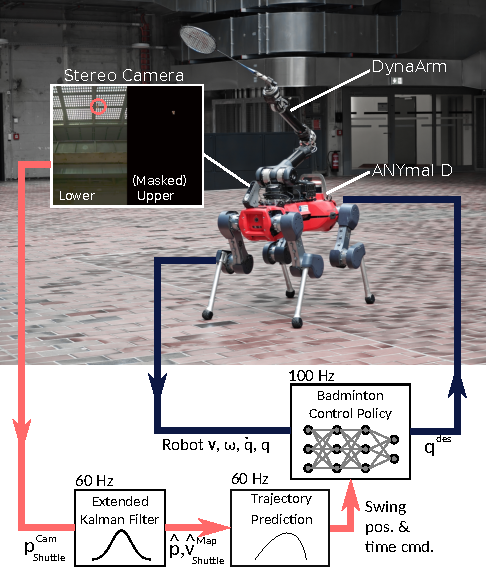
\includegraphics[width=0.5\textwidth]{Figures/SystemOverview/overview2.pdf}
    \caption{\textbf{System overview. } The legged mobile manipulator consists of a quadrupedal base and a dynamic arm. We additionally mounted a stereo camera with global shutters. The robot controller system receives the shuttle position computed in the camera frame, predicts the interception position, and feeds it to the RL policy along with the robot proprioception observations. The policy controls all 18 robot drives by producing joint commands.}
    \label{fig:overview}
    
    % \vspace{-1.5em}
\end{figure}
